%------------------------------
\begin{figure*}[t!]
  \centering
  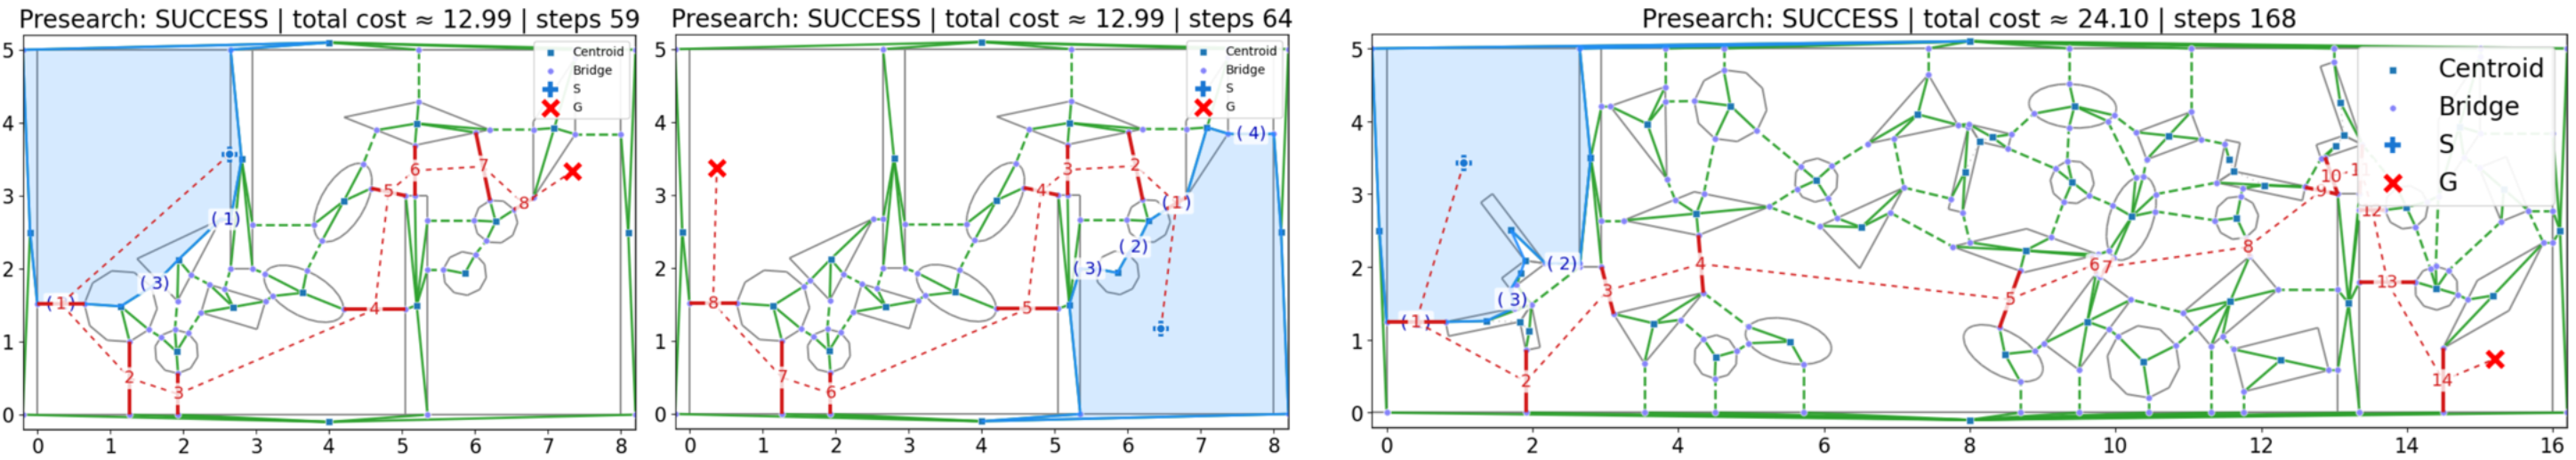
\includegraphics[width=0.95\linewidth]{figures/presearch.png}% or {presearch.pdf}
  \vspace{-0.15in}
\caption{
Illustration for {the ranking of potential gaps.}
Each panel shows the WCCG with the current face (light blue).
The algorithm (i) extracts the frontier loop from BugPlanner,
(ii) enumerates candidate bridge--bridge gaps on the loop,
(iii) assigns local first-hop ranks (blue numbers),
and (iv) simulates a short presearch to predict the full gap-crossing sequence (red numbers).
\textbf{Top}: start and goal swapped in the same map give symmetric
sequences with cost $12.99$;
\textbf{Right}: a larger map with about 30 obstacles produces a 14-gap sequence
with cost $24.10$.
}
  \label{fig:presearch}
   \vspace{-4mm}
\end{figure*}
%------------------------------
%==============================================
\subsection{W--Clearance Connectivity Graph}\label{subsec:wccg}

The feasibility of routing the vehicle reduces to whether a width-$W$ corridor 
connects $\mathbf{s}_\texttt{V}^{\texttt{S}}$ and $\mathbf{s}_\texttt{V}^{\texttt{G}}$. 
We introduce a W--Clearance Connectivity Graph (WCCG; Fig.~\ref{fig:wccg}) 
that encodes obstacle adjacencies under clearance $W$ and enables fast connectivity queries. 
Constructed directly from geometry (rather than grids/roadmaps), 
it avoids discretization error and remains consistent—crucial because connectivity is checked repeatedly 
during planning.

\subsubsection{Graph Construction}
The WCCG is built by decomposing each movable obstacle
$\Omega_m\in\boldsymbol{\Omega}$ into convex components. From each component
$C$, a centroid node $v_c$ is created. When two components $C_u$ and $C_v$
have closest points $p_u\in C_u$ and $p_v\in C_v$ with distance less than $W$, 
bridge nodes are added at $p_u$ and $p_v$. These bridge nodes are
connected by a bridge--bridge edge, annotated with the corresponding gap width
$w_{uv}\triangleq\|p_u-p_v\|$, and further linked back to their centroids with
centroid--bridge edges. Narrow passages with $w_{uv}<W$ are explicitly marked
as potential bottlenecks. The resulting graph is defined below:
\begin{equation}\label{eq:wccg}
\mathcal{G}_W\triangleq(\mathcal{V},\; \mathcal{E}_c\cup\mathcal{E}_b),
\end{equation}
where $\mathcal{V}$ contains all centroid and bridge nodes;
$\mathcal{E}_c$ is the set of centroid--bridge edges; and $\mathcal{E}_b$ the
set of bridge--bridge edges annotated by widths $w_{uv}$.

\subsubsection{Connectivity Criterion}\label{subsubsec:bugplanner}
Once $\mathcal{G}_W$ has been constructed, connectivity queries can be
performed without explicitly computing a geometric path. A frontier-tracing
procedure, similar to the BugPlanner~\cite{McGuireCroonTuyls2019}, starts from the vehicle start
$\mathbf{s}_\texttt{V}^{\texttt{S}}$, casts a ray toward the goal
$\mathbf{s}_\texttt{V}^{\texttt{G}}$, and explores the encountered loop of
frontier edges. If a valid exit is discovered, the process continues until the
goal is reached; otherwise a blocking cycle is returned. Successful execution
produces a skeleton $\Sigma$, which is an ordered sequence of centroid and
bridge nodes that certifies $\mathbf{s}_\texttt{V}^{\texttt{S}}$ and
$\mathbf{s}_\texttt{V}^{\texttt{G}}$ lie in the same connected face.
Let the $W$--clear free space be
$\mathcal{F}_W\triangleq\mathbb{R}^2\setminus(\mathcal{O}\oplus\mathbb{B}_{W/2})$,
where $\oplus$ denotes Minkowski addition and $\mathbb{B}_{W/2}$ is a closed
disk of radius $W/2$. A complete criterion for existence of a $W$--clear path
$\mathcal{P}^W_\texttt{V}$ is defined as:
\begin{equation}\label{eq:wccg_criterion}
\begin{aligned}
&\exists\,\mathcal{P}^W_\texttt{V}\subset\mathcal{F}_W:\
  \mathbf{s}_\texttt{V}^{\texttt{S}}\leadsto\mathbf{s}_\texttt{V}^{\texttt{G}} \Longleftrightarrow\
  \Big{\{}\mathbf{s}_\texttt{V}^{\texttt{S}},\mathbf{s}_\texttt{V}^{\texttt{G}}
  \ \text{belong to the} \\
  & \text{same face of }\mathcal{G}_W; \;\mathbb{B}_{W/2}(\mathbf{s}_\texttt{V}^{\texttt{S}}),
  \,\mathbb{B}_{W/2}(\mathbf{s}_\texttt{V}^{\texttt{G}})\subset\mathcal{F}_W\Big{\}},
\end{aligned}
\end{equation}
where $\mathbb{B}_{W/2}(\cdot)$ denotes a disk of radius $W/2$ centered at the
argument. This aligns with~\eqref{eq:wclear} for the external vehicle.

\subsubsection{Skeleton to Path}
The skeleton~$\Sigma$, the output of the previous step,
is an ordered sequence of centroid and bridge nodes connected by frontier
edges in $\mathcal{G}_W$. This skeleton serves as a compact certificate that
$\mathbf{s}_\texttt{V}^{\texttt{S}}$ and $\mathbf{s}_\texttt{V}^{\texttt{G}}$
lie in the same connected face. Given as input the skeleton $\Sigma$, together
with $\mathcal{G}_W$, the clearance $W$, and the endpoint disks
$\mathbb{B}_{W/2}(\mathbf{s}_\texttt{V}^{\texttt{S}})$ and
$\mathbb{B}_{W/2}(\mathbf{s}_\texttt{V}^{\texttt{G}})$, the output is an explicit
$W$--clear path $\mathcal{P}^W_\texttt{V}$. This path is constructed by sliding
each skeleton segment along the boundary of the inflated obstacles, offsetting
slightly inward into $\mathcal{F}_W$, and attaching short connectors inside the
endpoint disks. The resulting $\mathcal{P}^W_\texttt{V}$ remains in
$\mathcal{F}_W$, preserves the homotopy of $\Sigma$, and guarantees clearance of
at least $W$.


\begin{remark}\label{remark:wccg}
  The proposed WCCG differs from sampling- and grid-based planners in two key aspects:
  (I) It avoids discretization of $\mathcal{W}$ and is therefore free from
  resolution-induced errors;
  (II) It relies purely on geometry, which makes
queries highly efficient. These two features are crucial, since connectivity
checks and clearance tests are invoked many times within the hybrid
planner described in the sequel. \hfill$\blacksquare$
\end{remark}





%% \begin{algorithm}[t!]
%% \small
%% \caption{BugPlanner for $W$-width connectivity (skeleton witness)}
%% \label{alg:bugplanner}
%% \DontPrintSemicolon
%% \SetKwInOut{Input}{In}\SetKwInOut{Output}{Out}
%% \Input{$\mathbf{s}^{\texttt{S}}$, $\mathbf{s}^{\texttt{G}}$, WCCG}
%% \Output{if connected: skeleton $\Sigma$; else: frontier loop $\mathcal{L}$}
%% $P\leftarrow\mathbf{s}^{\texttt{S}}$, $\Sigma\leftarrow[\ ]$\;
%% \While{true}{
%%   \If{segment $P\mathbf{s}^{\texttt{G}}$ hits no edge}{\Return $\Sigma \cup \{\texttt{straight}(P,\mathbf{s}^{\texttt{G}})\}$}
%%   Build loop $\mathcal{L}$ by angle-follow from the hit edge; append traversed edges to $\Sigma$\;
%%   \If{$\mathrm{parity}(\mathcal{L},\,\mathbf{s}^{\texttt{S}}\mathbf{s}^{\texttt{G}})$ is odd}{\Return $(\emptyset,\mathcal{L})$}
%%   Choose exit $e$ on $\mathcal{L}$ (outward normal $\to\,\mathbf{s}^{\texttt{G}}$); append arc to $\Sigma$; $P\leftarrow e$ (tiny bias)\;
%% }
%% \end{algorithm}
